{
\setbeamertemplate{footline}{}
\setbeamertemplate{sidebar right}{\llap{
\includegraphics[width=\paperwidth,height=\paperheight]{BG_upper}}}
\begin{frame}[c]%{\phantom{title page}}
\phantom{title page}
 \titlepage
\end{frame}
\addtocounter{framenumber}{-1}

}


\begin{frame}{Unsupervised Learning of How to Perform a Task}
  We (humans \& robots) are using recipe books since 9th century.
\begin{columns}
  \begin{column}[T]{5.5cm}
    \centering
    {\bf Humans}
    \begin{itemize}
      	{\setbeamertemplate{itemize item}[good]
        \item Expert curated solution}
        {\setbeamertemplate{itemize item}[bad]
        \item Generally a single recipe is available}
        {\setbeamertemplate{itemize item}[bad]
        \item Lacks visual information}
        {\setbeamertemplate{itemize item}[bad]
        \item Even if the visual information exists, only a single view with some important parts are occluded}
    \end{itemize}
  \end{column}
  \begin{column}[T]{5.5cm}
    \centering
    {\bf Robots [1,2]}
    \begin{itemize}
{\setbeamertemplate{itemize item}[bad]
\item Assume common sense knowledge}
{\setbeamertemplate{itemize item}[bad]
\item Ambigous language}
{\setbeamertemplate{itemize item}[bad]
\item Requires lots of supervision for (partially) succesfull operation.}
    \end{itemize}
  \end{column}

\end{columns}
\vfill
\tiny
[1] M. Bollini, J. Barry, and D. Rus, \emph{BakeBot: Baking Cookies with the PR2}, IROS 2011 \newline
[2] M. Beetz, U. Klank, I. Kresse, A. Maldonado, L. Mosenlechner, D. Pangercic, T. Ruhr and M. Tenorth, \emph{Robotic Roommates Making Pancakes}, Humanoids 2011
\normal
\end{frame}

\begin{frame}{Community Driven Solution}
YouTube already has large-scale, multi-modal recipes (eg 281,000 video with speech for \emph{how to tie a bow tie}). For a given query,
\begin{itemize}
  \item It has multiple ways of performing the task
  \item It has (automtically generated) language information.
  \item Videos cover variety of environment conditions, camera angles, close-up etc.
\end{itemize}
However,
\begin{itemize}
  \item A typical human will not watch 281,000 videos.
  \item A robot needs a structured information.
\end{itemize}
\vspace{0.7cm}
\textbf{If we can automatically find the activities/steps, we can bring a structure to the videos and summarize 281,000 videos. Win-win scenario for both robots and humans.}
\end{frame}


\begin{frame}{Related Work}
  \begin{itemize}
  \item Recipe Understanding
    \begin{itemize}
      \item Cooking with Semantics [J Malmaud et al.]: Parsing text recipes and learning affordances
      \item What's Cookin'?  [J Malmaud et al.]: Matching a text recipe to the subtitles
      \item BakeBot: Baking Cookies with the PR2 [M.Beetz et al.] Extracting a plan out of a recipe
    \end{itemize}
  \item Multi-Modal Activity Detection/Recognition
    \begin{itemize}
      \item Grounding Action Descriptions in Videos [M. Regneri]: Can visual data help semantic understanding of sentences?
      \item Language Learning from Videos [H. Yu], YouTube2Text [S. Guadarrama], MPII Movie Description [A. Rohrbach]: Generating captions for video clips.
    \end{itemize}
  \end{itemize}
\end{frame}

\begin{frame}{Related Work-2}
  \begin{itemize}
    \item Video Summarization
    \begin{itemize}
      \item Reconstructing Storyline Graphs [G. Kim]: Recovering the temporal dynamics of large photo collection.
      \item Understanding Videos, Constructing Plots [A. Gupta]: Given activity labels, summarizing all videos as a graph.
    \end{itemize}
  \end{itemize}
  \vspace{5mm}
  \begin{center}
  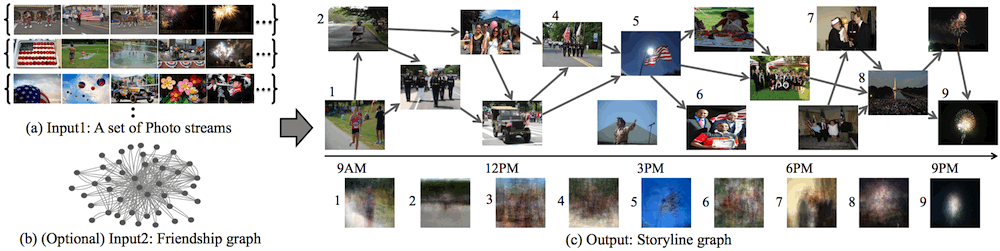
\includegraphics[width=0.8\textwidth]{storygraph}
  \end{center}
\end{frame}

\begin{frame}{Challanges-Noise}
  These are part of top 25 results when the query is How to make a milkshake?
\\  \vspace{5mm} \\
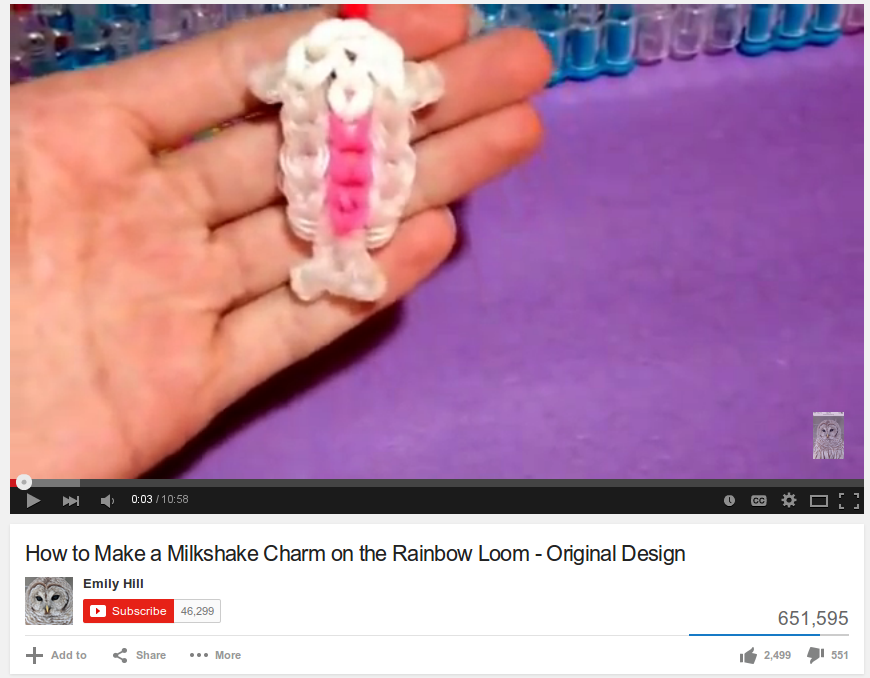
\includegraphics[width=0.33\textwidth]{troll1}
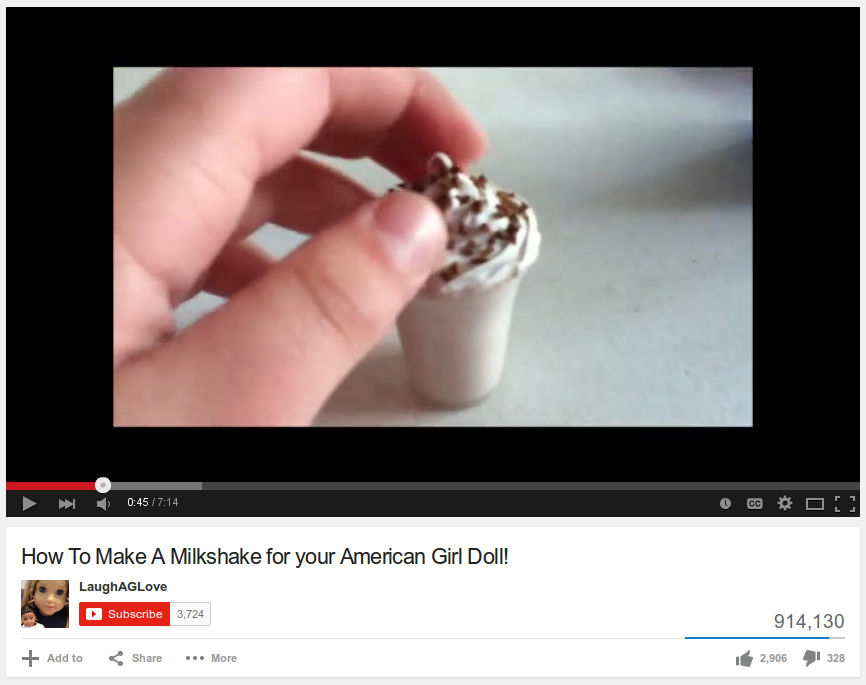
\includegraphics[width=0.33\textwidth]{troll2}
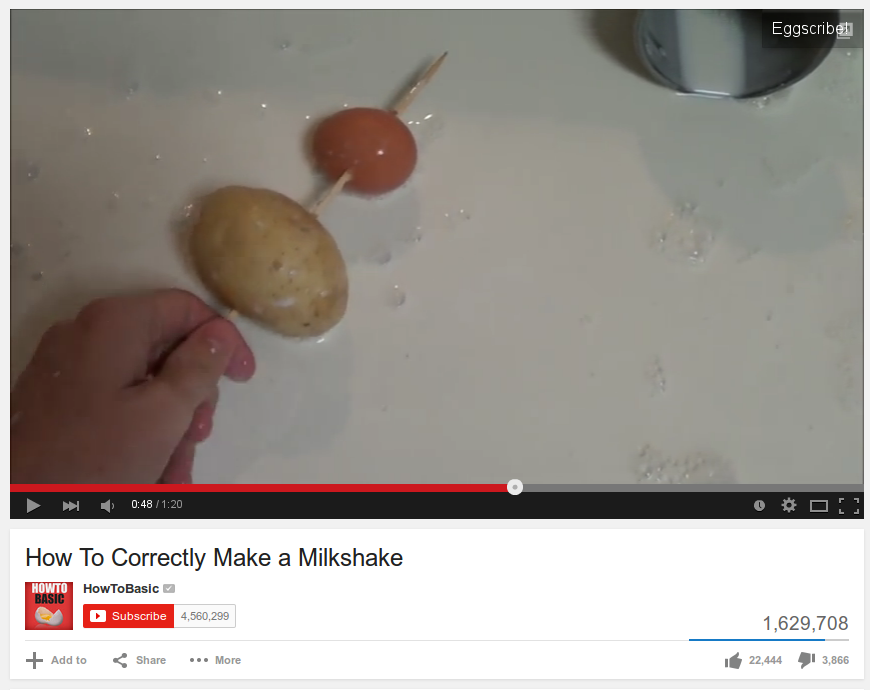
\includegraphics[width=0.33\textwidth]{troll3}
\end{frame}


\begin{frame}{Challanges-Visual Variety}
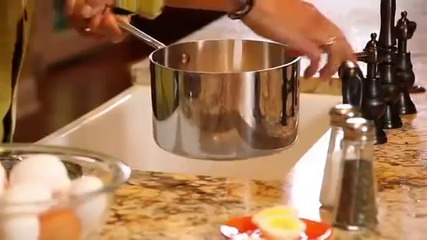
\includegraphics[width=0.33\textwidth]{water1}
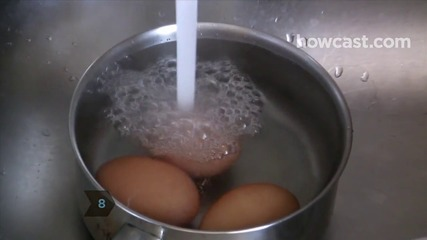
\includegraphics[width=0.33\textwidth]{water2}
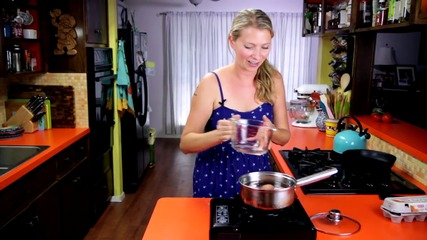
\includegraphics[width=0.33\textwidth]{water3}
\end{frame}


\begin{frame}{Overview}
  \includegraphics[width=\textwidth]{algor}
\end{frame}

\begin{frame}{Collecting Data}
  \begin{itemize}
    \item For given a query, we download top 100 videos from YouTube.
    \item Each video has a language description ($D_i$), and we compute pairwise semantic distances by using Dice coefficients of n-grams ($n=2$)
    \item We compute the normalized cut as thresholding the result of; ($A_{i,j}=d(D_i,D_j)$)
    \[
    \argmax_{x \in [0,1]^{100}} \frac{x^TAx}{x^Tx}
    \]
    \item Resulting dominant cluster is used for the rest of the video.
  \end{itemize}
\end{frame}

\begin{frame}{Finding Objects}
  \begin{itemize}
    \item We generate object proposals ($P^1_{i},\ldots,P^R_{i}$) for each frame ($t$) of each video ($i$).
    \item We cluster the proposals in order to find objects; let's say $x^p_{i,r}$ is $1$ if $p^{th}$ cluster, has $r^{th}$ proposal of $i^{th}$ video.
    \item We define the clustering problem as ($A$ is pairwise distance matrix with fc7 AlexNet features)
    \[
    \argmax_{x}  \sum_{i} \frac{x_{i,\cdot}^TA_i x_{i,\cdot}}{x_{i,\cdot}^Tx_{i,\cdot}} +
   \sum_{i}\sum_{j \in \mathcal{N}_k(i)} \frac{x_{i,\cdot}^TA_{ij}x_{j,\cdot}}{x_{i,\cdot}^T \mathds{1} \mathds{1}^Tx_{j,\cdot}}
    \]
    \item This maximum of this function is a cut over proposals which all videos agree on and has maximum normalized total similarity within cluster.
    \item This function is quasi-convex and can be maximized by using sub-gradient method.
  \end{itemize}
\end{frame}

\begin{frame}{Some Visual Objects}
  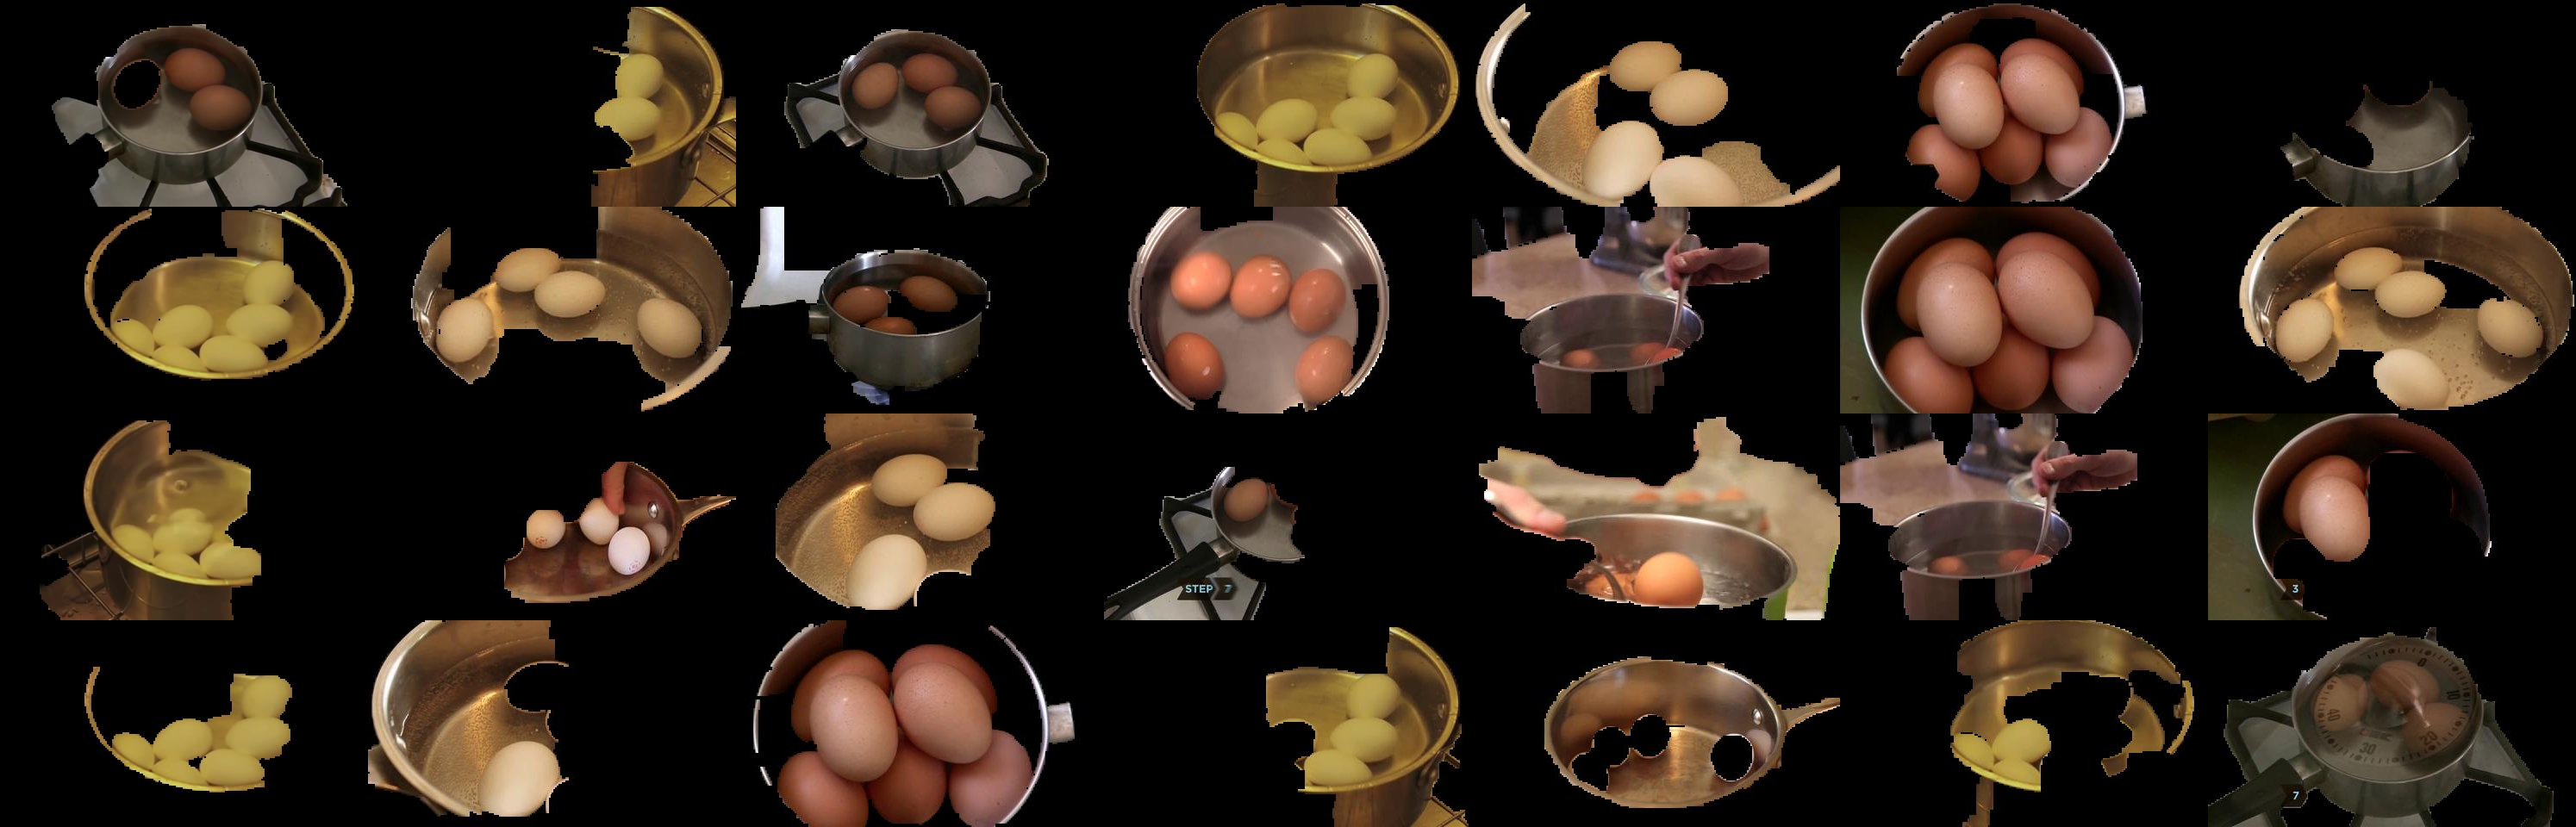
\includegraphics[width=\textwidth]{im10.png}
  \\
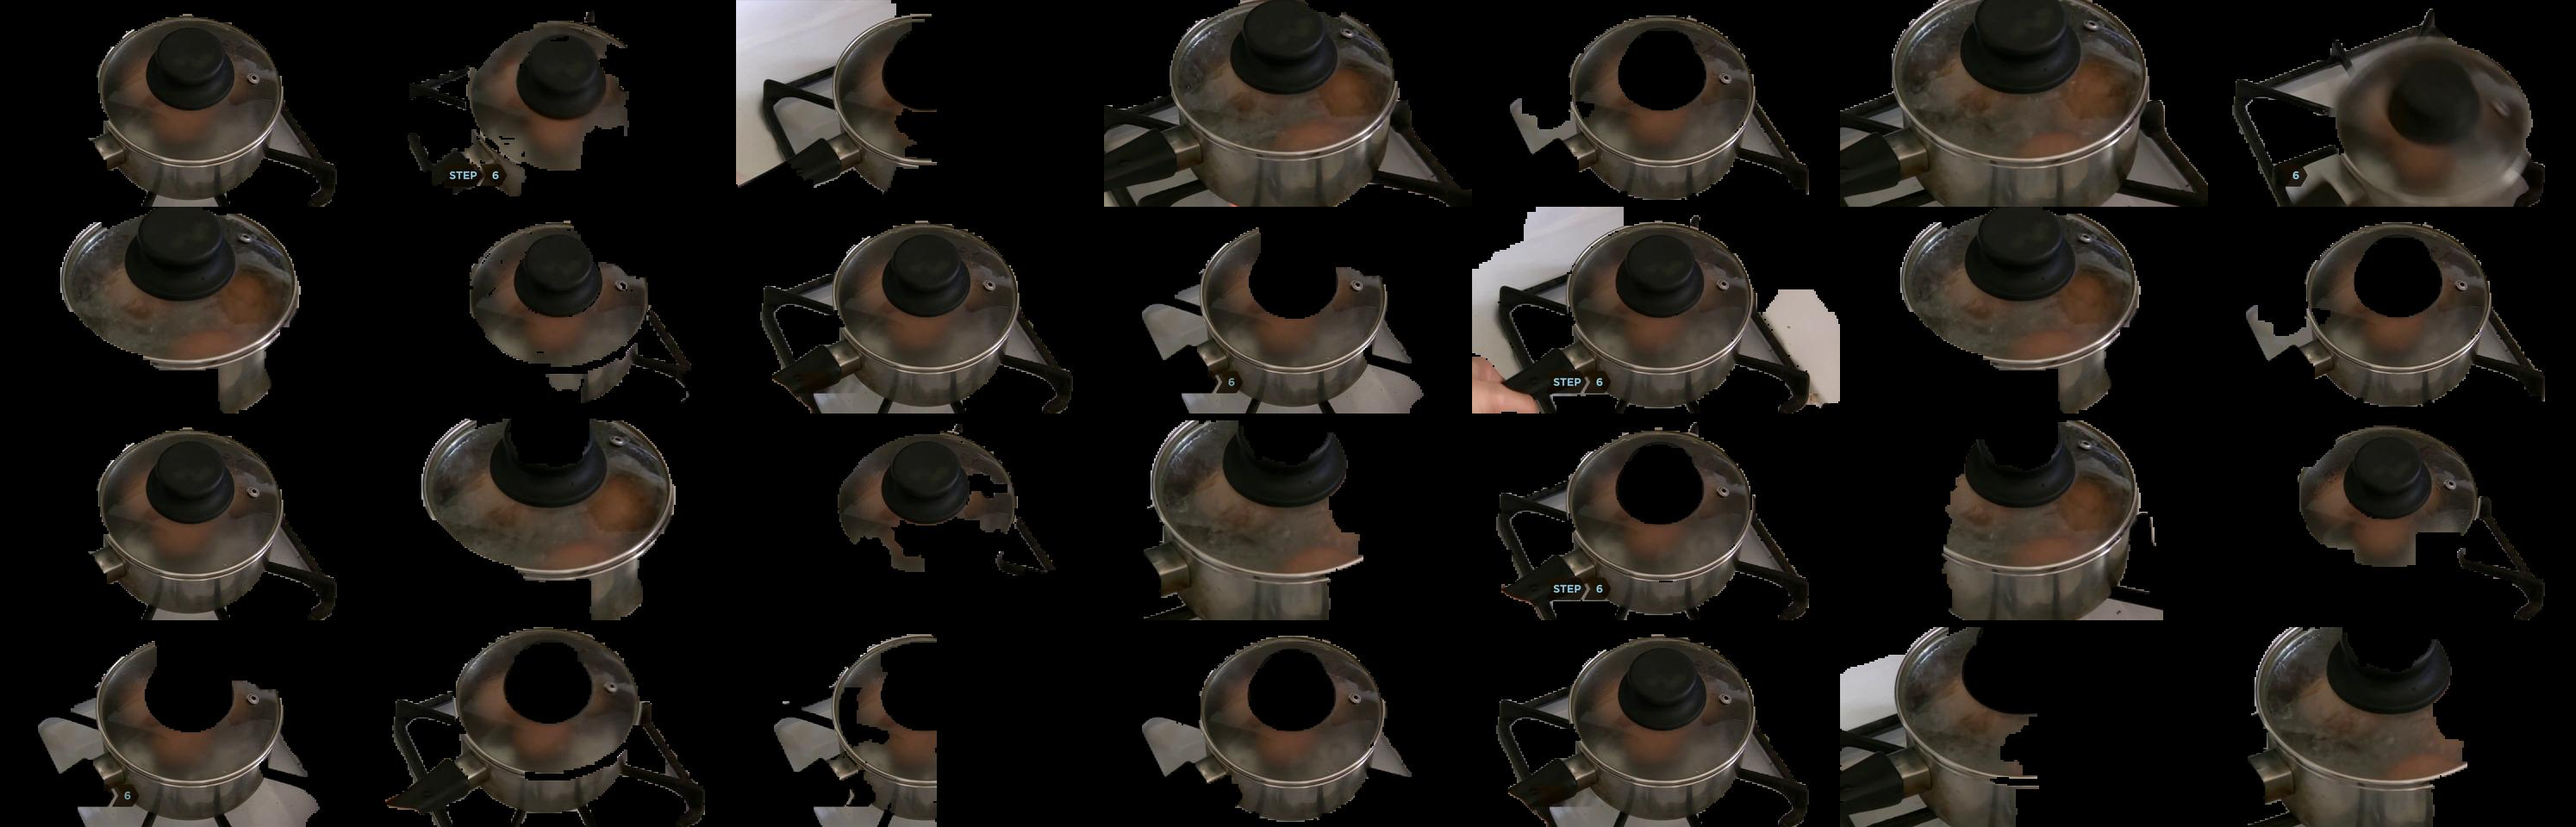
\includegraphics[width=\textwidth]{im9.png}
\end{frame}

\begin{frame}{Some Visual Objects-2}
  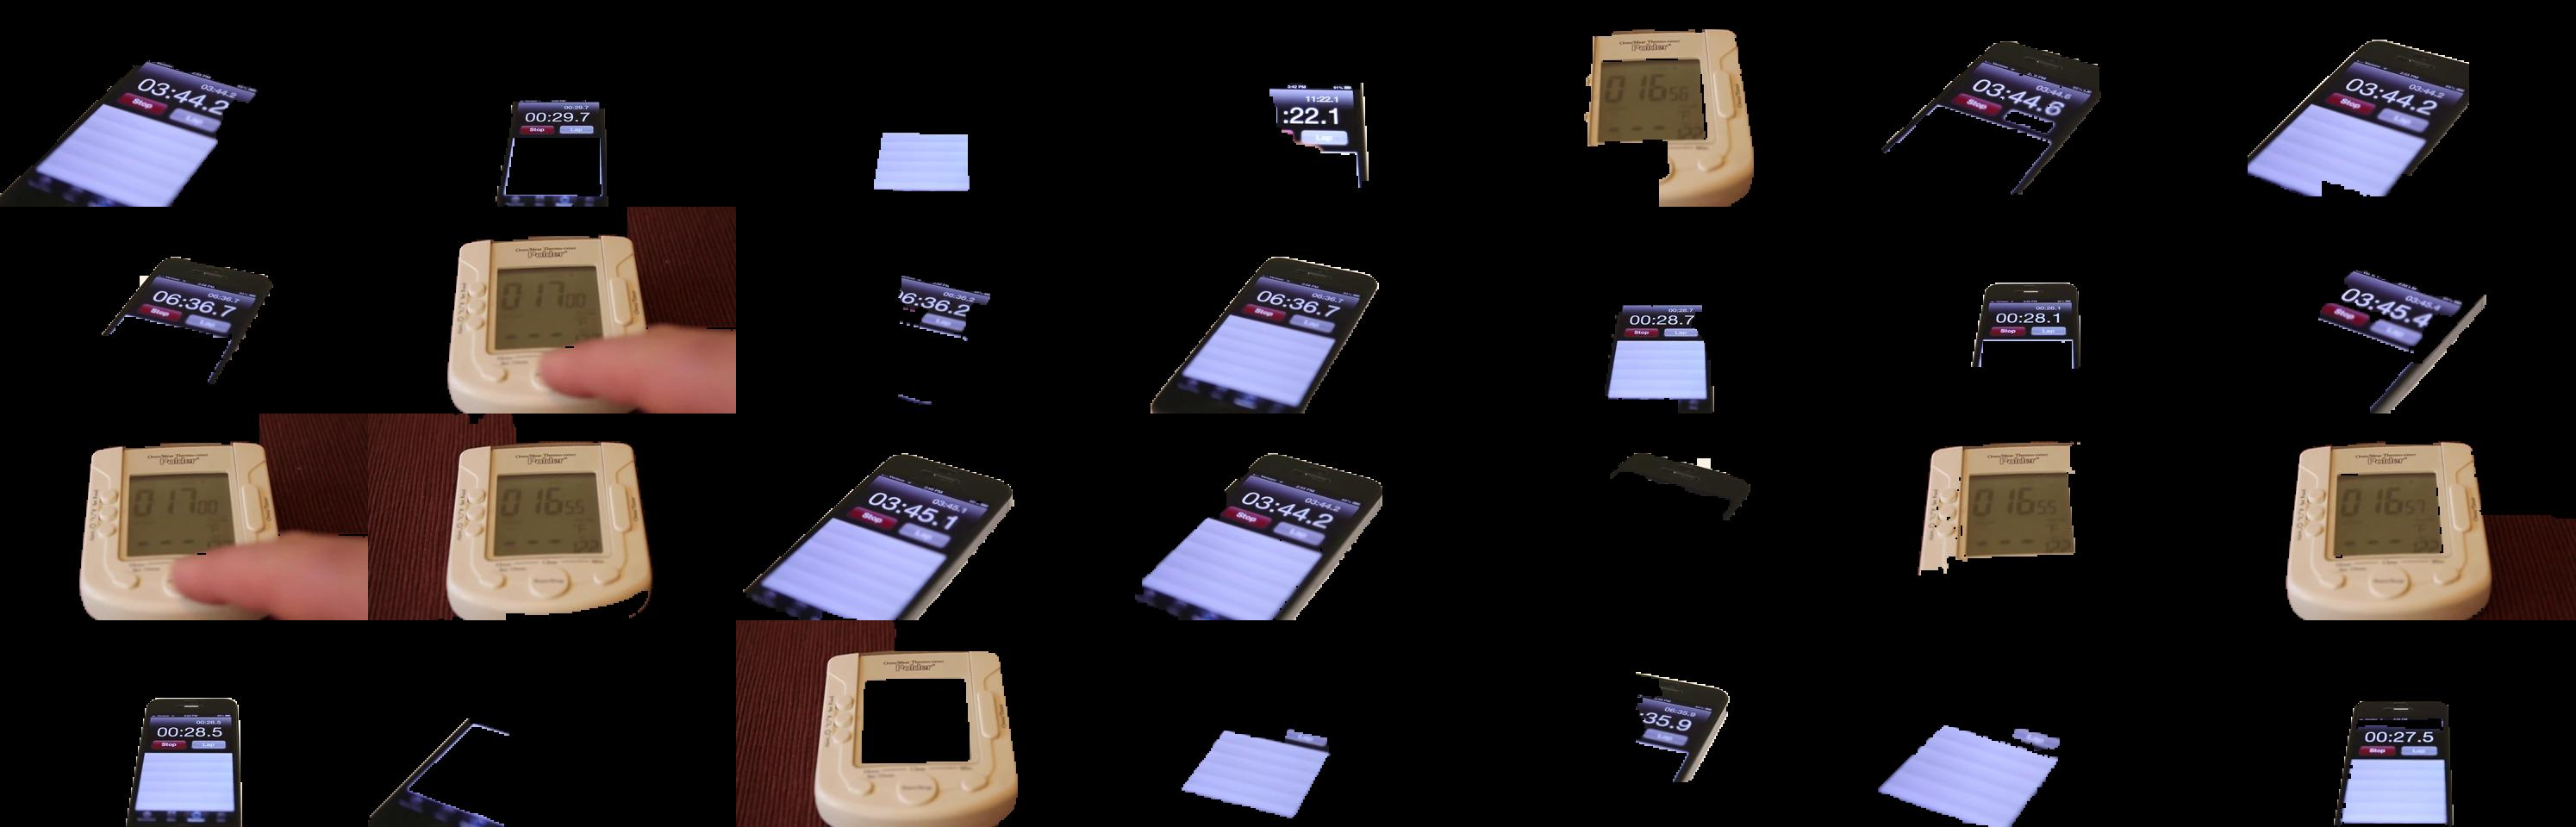
\includegraphics[width=\textwidth]{im8.png}
  \\
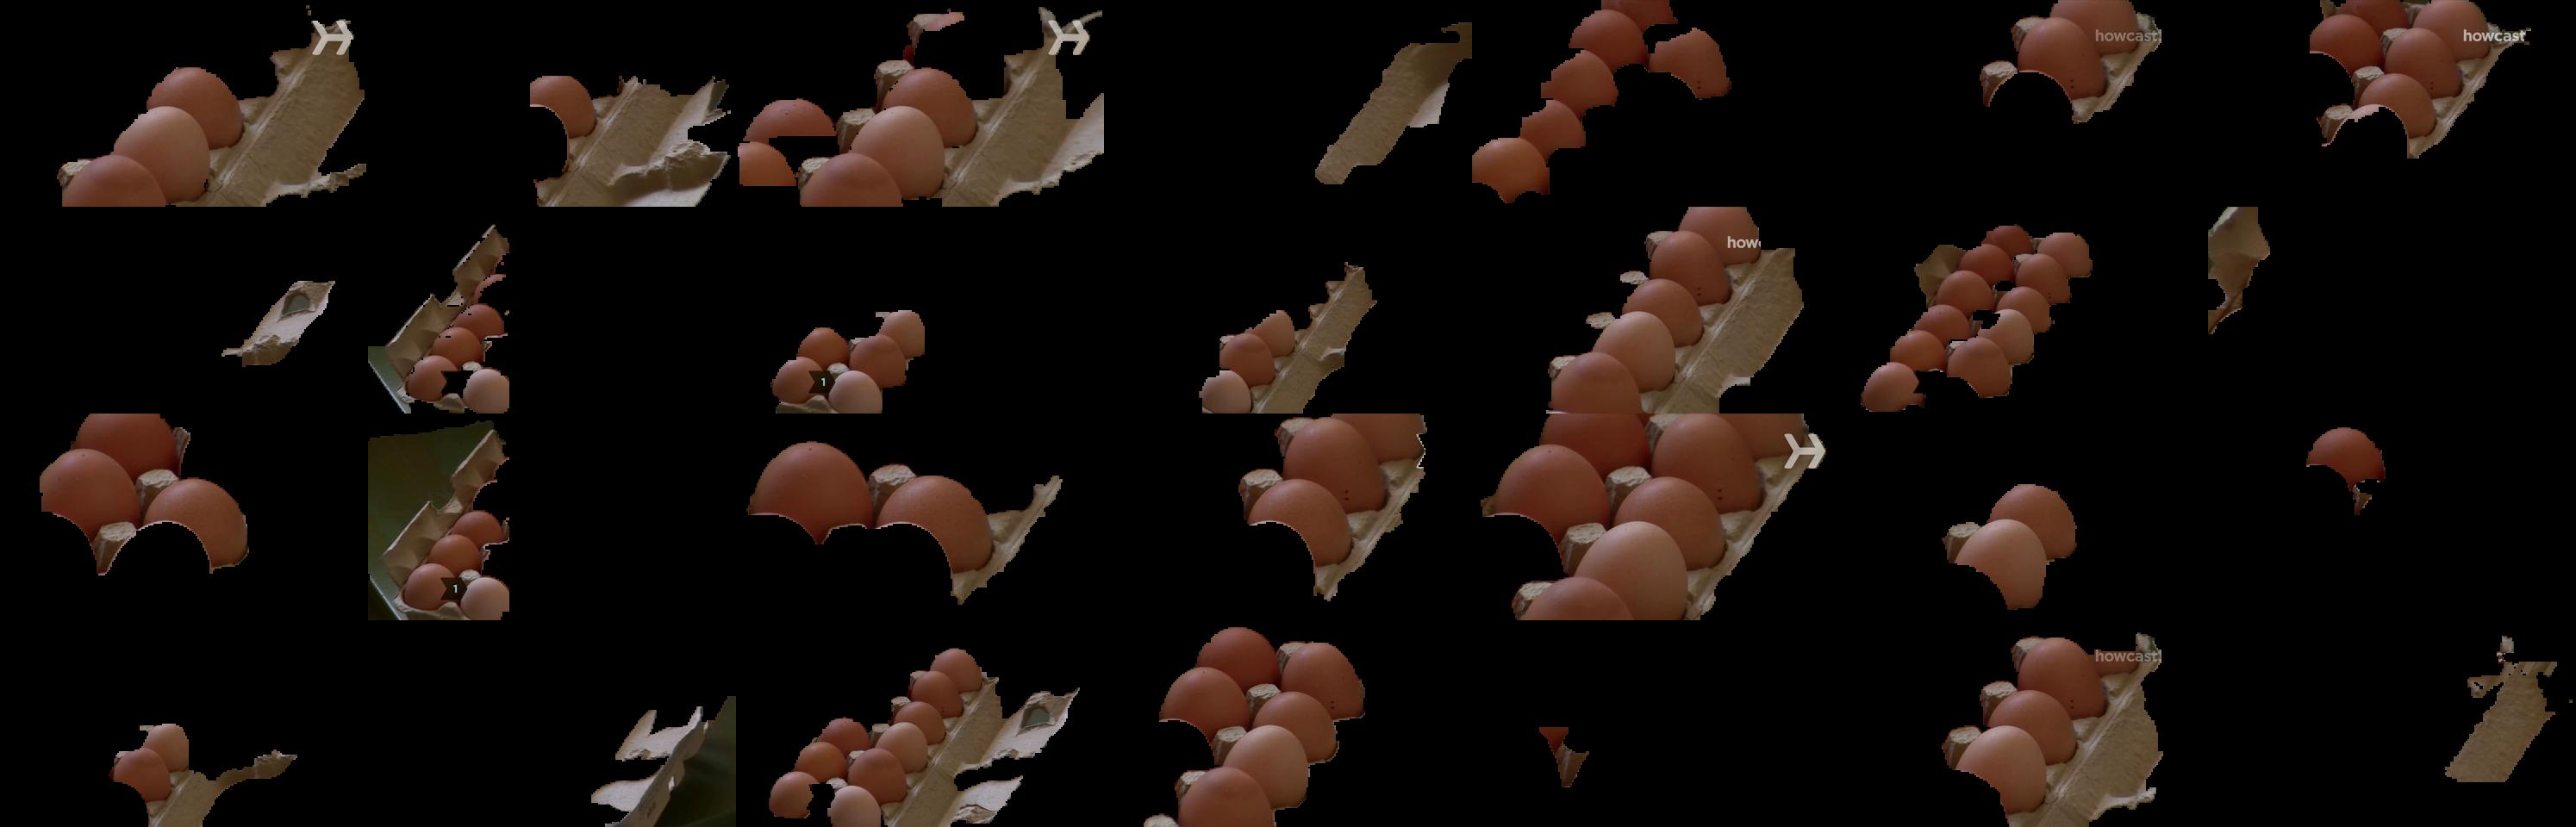
\includegraphics[width=\textwidth]{im7.png}
\end{frame}

\begin{frame}{Some Visual Objects-3}
  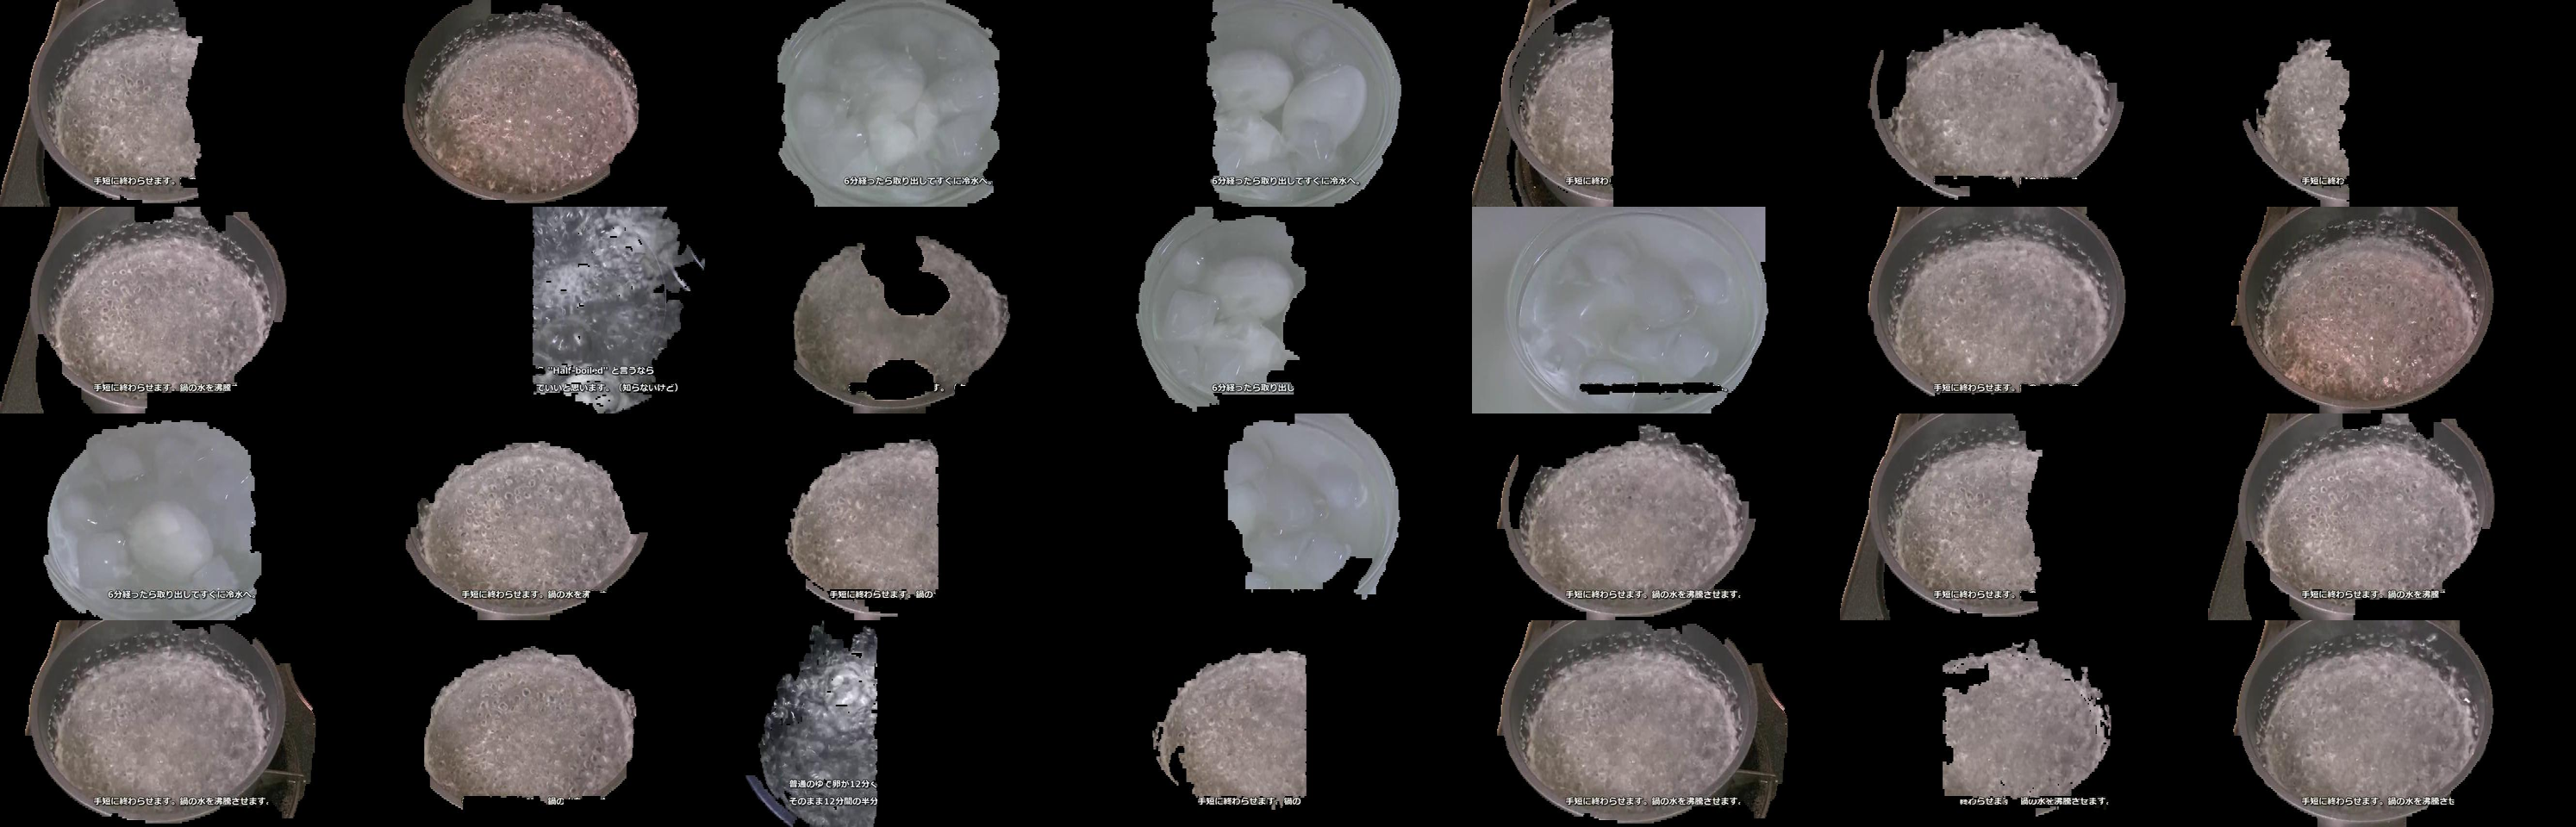
\includegraphics[width=\textwidth]{im5.png}
  \\
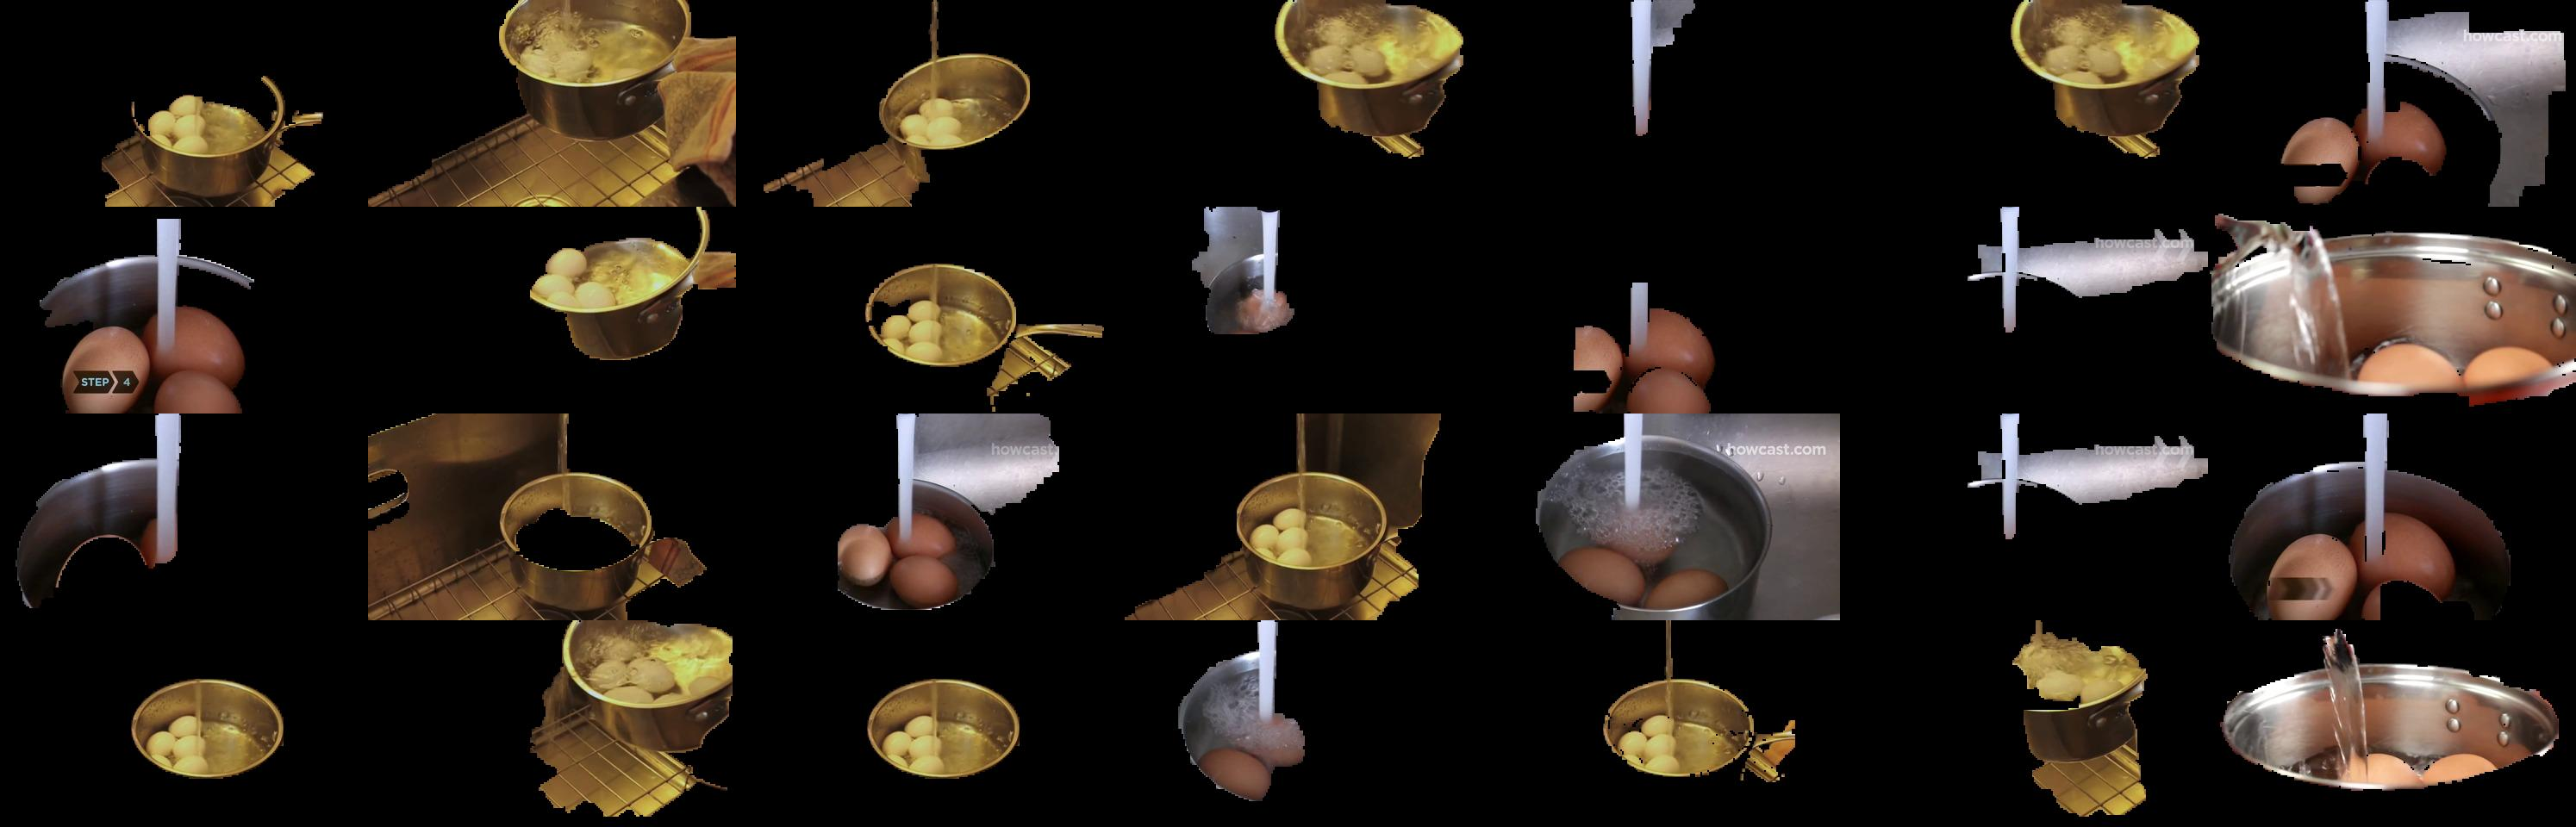
\includegraphics[width=\textwidth]{im0.png}
\end{frame}

\begin{frame}{Finding Salient Words}
  \begin{itemize}
    \item We concatanate all subtitles and compute the frequency of each word ($f_t$).
    \item For each selected word, we compute the frequency of each word in NYTimes corpus ($f_d$).
    \item We choose the $K$ most frequent words with property $f_t>f_d$.
  \end{itemize}
\end{frame}


\begin{frame}{Salient Words}
First 50 salient words:
\\ \vspace{1cm} \\
sort, place, water, egg, bottom, fresh, pot, crack, cold, cover, time, overcooking, hot, shell, stove, turn, cook, boil, break, pinch, salt, peel, lid, point, haigh, rules, perfectly, hard, smell, fast, soft, chill, ice, bowl, remove, aside, store, set, temperature, coagulates, yolk, drain, swirl, shake, white, roll, handle, surface, flat
\end{frame}



\begin{frame}{Learning Recipes}
\begin{itemize}
  \item Each activity ($\theta_k$) is represented as Binomial r.v. over visual objects and Drichlet r.v. over language words.
  \item Each video choose set of activities ($f_i$) with likelihoods ($w_k$) following the Indian Buffet Process.
  \end{itemize}

\begin{center} 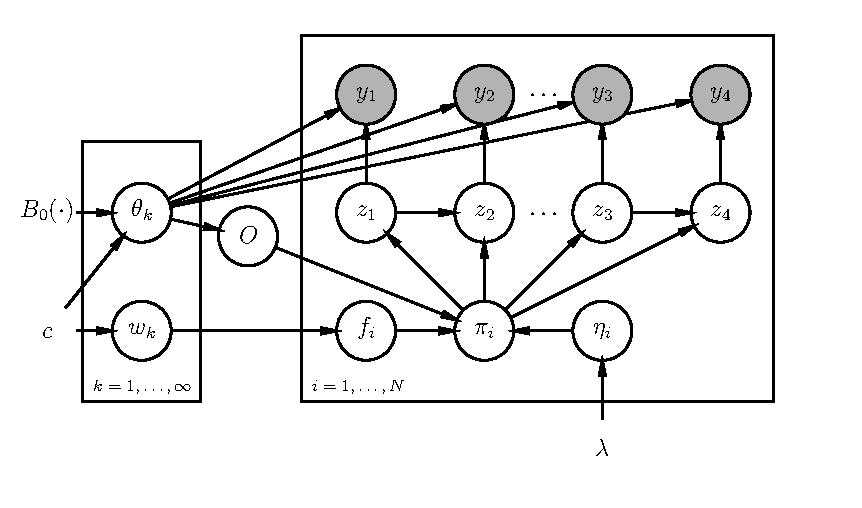
\includegraphics[width=0.8\textwidth]{classic} \end{center}
\end{frame}

\begin{frame}{Learning Recipes - 2}
\begin{itemize}
  \item Some activities impose time ordering via $O$ e.g. activity 1 is always after activity 2 if $O_{1,2}=1$.
  \item Activities have prior transition probabilities ($\eta_i^{m,n}$ is the transition prob from activity $m$ to $n$, $\eta_i^{m,\cdot}$ follows a Drichlet r.v.
%  \item We represent each frame ($y_i$) as binary vector of occurance of visual objects and bag of language words.
%  \item Each video choose set of activities ($f_i$) with likelihoods ($w_k$) following the Indian Buffet Process.
  \end{itemize}

\begin{center} 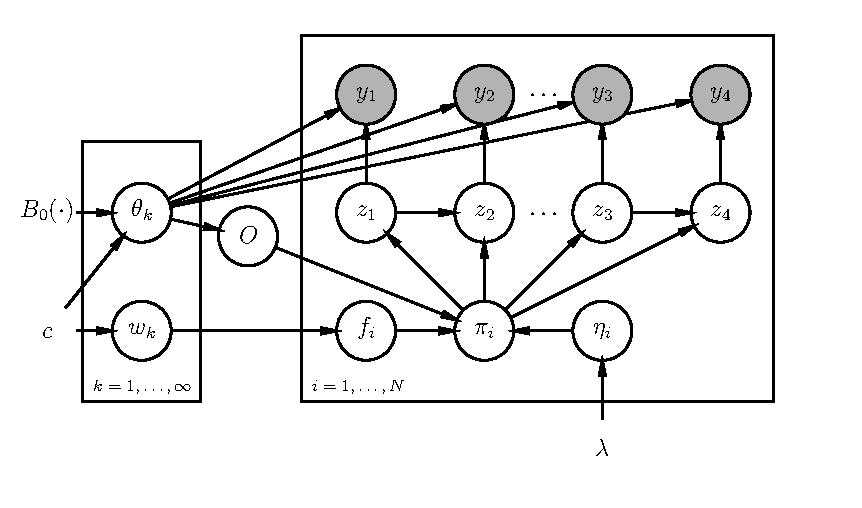
\includegraphics[width=0.8\textwidth]{classic} \end{center}
\end{frame}


\begin{frame}{Learning Recipes - 3}
\begin{itemize}
  \item Transition probabilities($\pi_i$) is normalized version of prior transition probabilities obeying selected activities and time orderings.
  \[
  \pi_i = \frac{f_i \otimes \eta_i \otimes O_{\cdot,i}}{\|f_i \otimes \eta_i \otimes O_{\cdot,i}\|}, \hspace{5mm}  \otimes \text{is elementwise product}
  \]
%
%  \item Each video choose set of activities ($f_i$) with likelihoods ($w_k$) following the Indian Buffet Process.
  \end{itemize}

\begin{center} 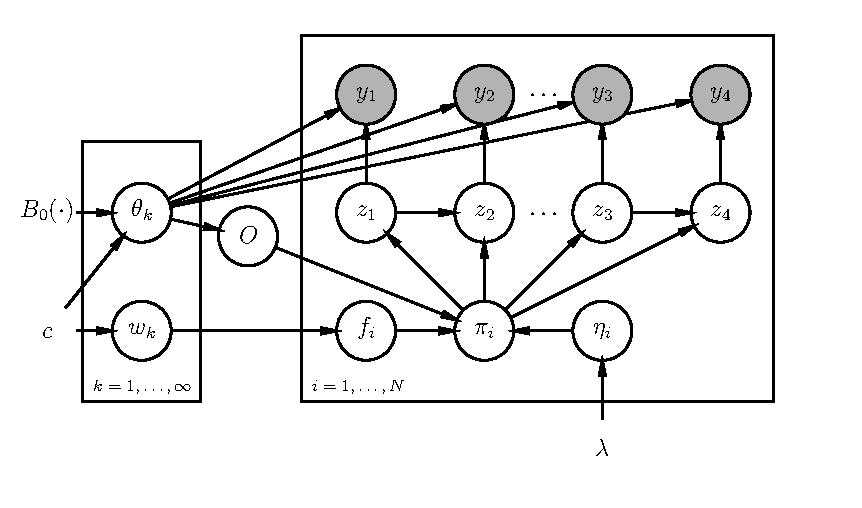
\includegraphics[width=0.8\textwidth]{classic} \end{center}
\end{frame}


\begin{frame}{Learning Recipes - 4}
\begin{itemize}
\item We represent each frame ($y_i$) as binary vector of occurance of visual objects and bag of language words.
\item $z_t$ is the activity of frame $t$ and it follows an HMM.
\end{itemize}
\begin{center} 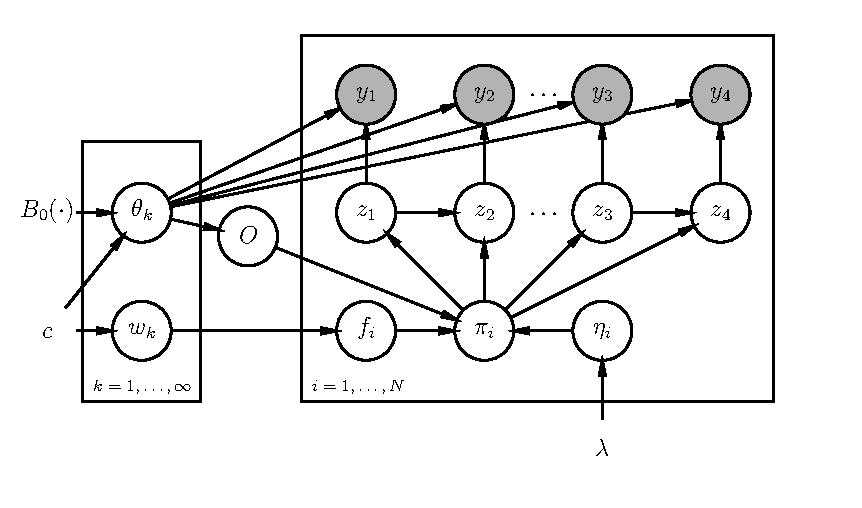
\includegraphics[width=0.8\textwidth]{classic} \end{center}
\end{frame}

\begin{frame}{Learning}
  \begin{itemize}
\item We use Metropolis–Hastings sampler for binary random variables and Gibbs sampler for the rest.
\item Time ordering matrix and IBP is sampled via data driven manner (details omitted).
\end{itemize}
\end{frame}



\begin{frame}{Preliminary Results}
\begin{itemize}
  \item We crawl the top 50 queries from the WikiHow.com and manually choose 25 out of them.
  \item For each query, we download 100 videos (total of 2500 videos, average length~7min, 80\% have ASR subtitles)
  \item For each recipe, we have 5 evaluation videos with temporal activity labels as well as the activity names.
  \item We run the full model for 95 videos with no label and test in the remaining 5. For the test set, we do not sample the activities.
  \item We compute average intersection-over-union for the temporal segmentation (best over all matchings).
\end{itemize}
\begin{center}
\begin{tabular}{cc}
  KMeans with Correct Number of States & 20.74\% \\
  HMM with Correct Number of States & 24.25\% \\
  Our Method & 54.68\%
\end{tabular}
\end{center}
\end{frame}

\begin{frame}{Discussion}
  \begin{itemize}
    \item Preliminary results suggest that the weak signal in the subtitles is powerful enough to recover activities.This can be used to scale-up activity detection algorithms.
    \item Activities are computed by using a generative model in other words we can have multiple/none activity in the same time.
    \item Integration of a recipe book is still an open problem and possibly a future work.
  \end{itemize}
\end{frame}

\begin{frame}{Dataset}
(How to)+Bake Boneless Skinless Chicken, Cook Steak in a Frying Pan, Make Jello Shots, Tell if Gold Is Real, Bake Chicken Breast, Hard Boil an Egg, Make Pancakes, Tie a Bow Tie
Broil Steak, Make a Grilled Cheese Sandwich, Make Scrambled Eggs, Tie a Tie, Clean a Coffee Maker, Make a Milkshake, Make Yogurt, Unclog a Bathtub Drain, Cook an Omelette,
Make a Smoothie, Poach an Egg, Cook Lobster Tails, Make Beef Jerky, Remove Gum from Clothes, Cook Ribs in the Oven, Make Ice Cream, Tell if an Egg is Bad
\end{frame}
